\documentclass{beamer}

\usepackage[beamer]{shortcut}
\graphicspath{{./images/}}

\def\biblio{
    \nobibliography{library}
    \def\biblio{}
}

\institute{Inria Saclay}
\author{Thomas Moreau}
\title{
    EBUL: Event-based Unsupervised Learning for Physiological Signals
}

\setbeamertemplate{title page}[frame]
\setbeamercovered{invisible}
% \def\extraLogo{\vskip-4em\includegraphics[height=8em]{logo_EBUL}}

\setlength\SizeLogoPage{8em}
\def\LOGOS{
% \includeLogos[1em]{logo_mind_big,logo_EBUL,logo_inria}\\[.5em]
    \hskip-1em
    \raisebox{-1.5em}{
\includegraphics[height=3em]{logo_inria}}
    % \hskip2em
    % \raisebox{-4em}{\includegraphics[height=8em]{logo_EBUL}}
    \hskip2em
    \raisebox{-2.5em}{\includegraphics[height=5em]{logo_cea}}\\[.5em]
}
\collaborators[]{Kick-off ANR 2023}

\newcommand{\fakecite}[1]{\textcolor{gray}{[{\color{linkcolor} #1}]}}

\begin{document}

\begin{frame}
    \titlepage
    % \biblio{}
\end{frame}

%------------------------------------------------------------------------------
{
\usebackgroundtemplate{
    \begin{picture}(400, 300)(45, 0)
        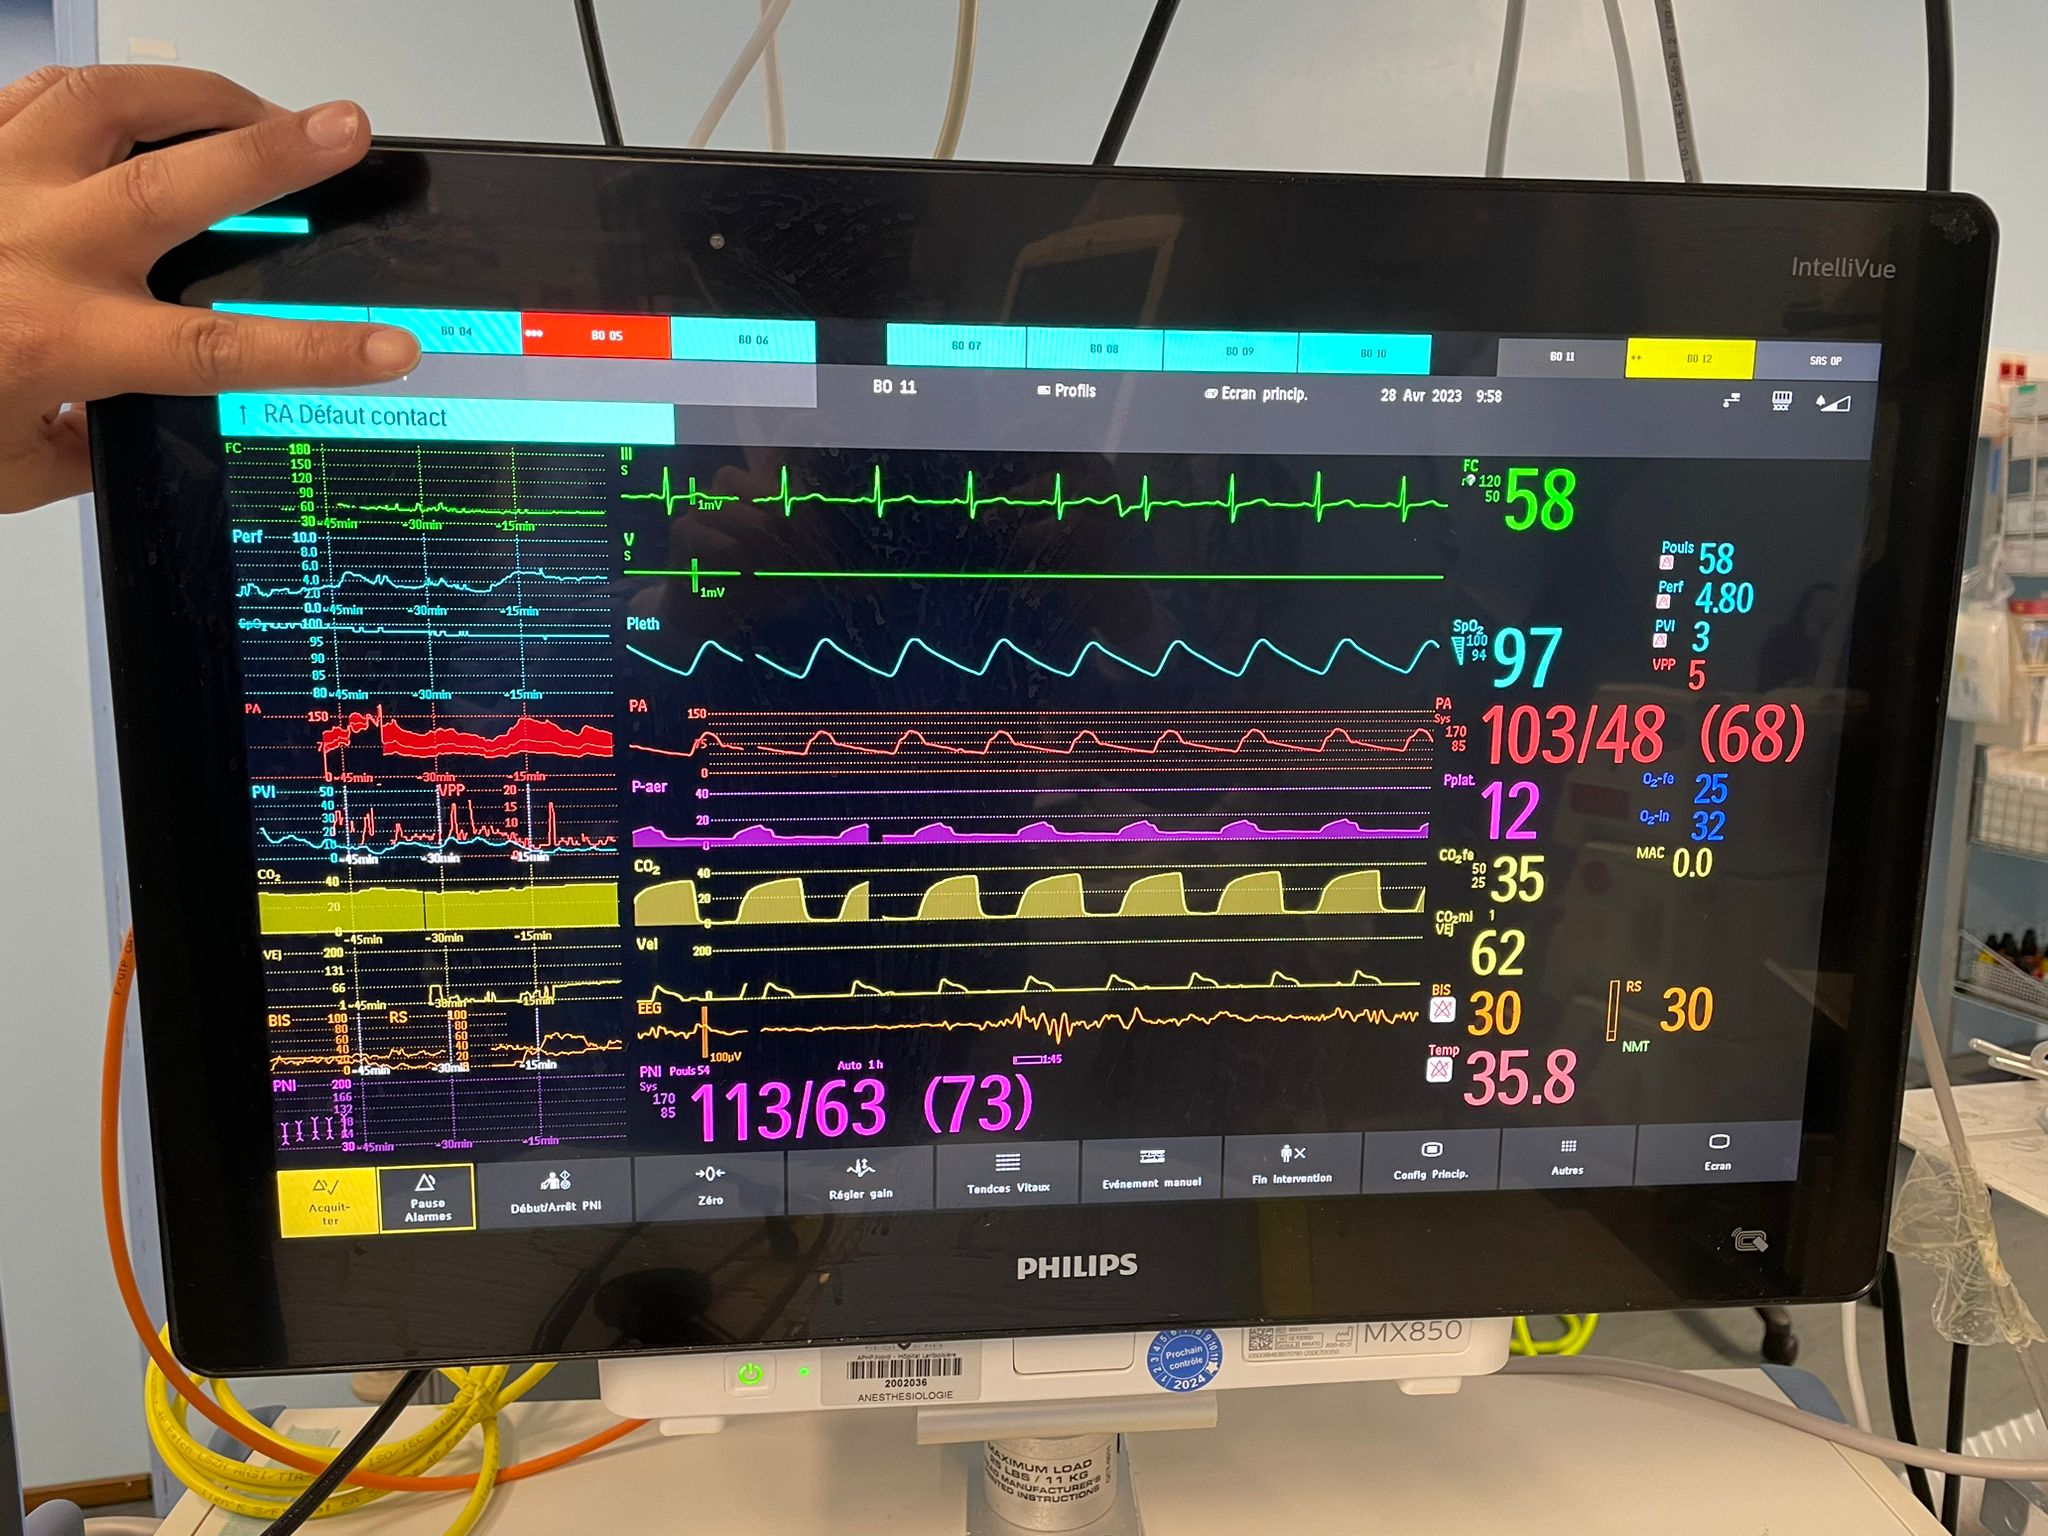
\includegraphics[
            width=1.16\paperwidth
        ]{GA_monitor_1}
    \end{picture}
}
\frame{
    \frametitle{General Anesthesia Monitoring}


    \begin{tikzpicture}[overlay, remember picture]
            \node[anchor=center, white, xshift=-32ex, yshift=-6em] at (current page.north) (ECG) {\highlight[shadow=false]{\Large \bf ECG}};
            \node[anchor=center, white, xshift=-13ex, yshift=-7.5em] at (current page.north) (ECG_head) {};
            \draw[->, very thick, white] (ECG.east) -- (ECG_head);

            \node[anchor=center, white, xshift=-32ex, yshift=-9.5em] at (current page.north) (Pleth) {\highlight[shadow=false]{\Large \bf Pleth.}};
            \node[anchor=center, white, xshift=-11ex, yshift=-10.5em] at (current page.north) (Pleth_head) {};
            \draw[->, very thick, white] (Pleth.east) -- (Pleth_head);

            \node[anchor=center, white, xshift=-32ex, yshift=-13.5em] at (current page.north) (Resp) {\highlight[shadow=false]{\Large \bf Resp.}};
            \node[anchor=center, white, xshift=-7ex, yshift=-15em] at (current page.north) (Resp_head) {};
            \draw[->, very thick, white] (Resp.east) -- (Resp_head);

            \node[anchor=center, white, xshift=-32ex, yshift=-16.5em] at (current page.north) (EEG) {\highlight[shadow=false]{\Large \bf EEG}};
            \node[anchor=center, white, xshift=-5ex, yshift=-17.5em] at (current page.north) (EEG_head) {};
            \draw[->, very thick, white] (EEG.east) -- (EEG_head);
            \node[anchor=north west, xshift=18ex, yshift=-6em] at (current page.north) {
                \highlight[shadow=false]{Indicators}
            };


            \node[anchor=south east, yshift=1em, xshift=-4ex] at (current page.south east) {
                \highlight[shadow=false]{\includegraphics[height=2em]{logo_aphp}}
            };

    \end{tikzpicture}
}
}


%------------------------------------------------------------------------------
{
\usebackgroundtemplate{
    \begin{picture}(400, 300)(45, 0)
        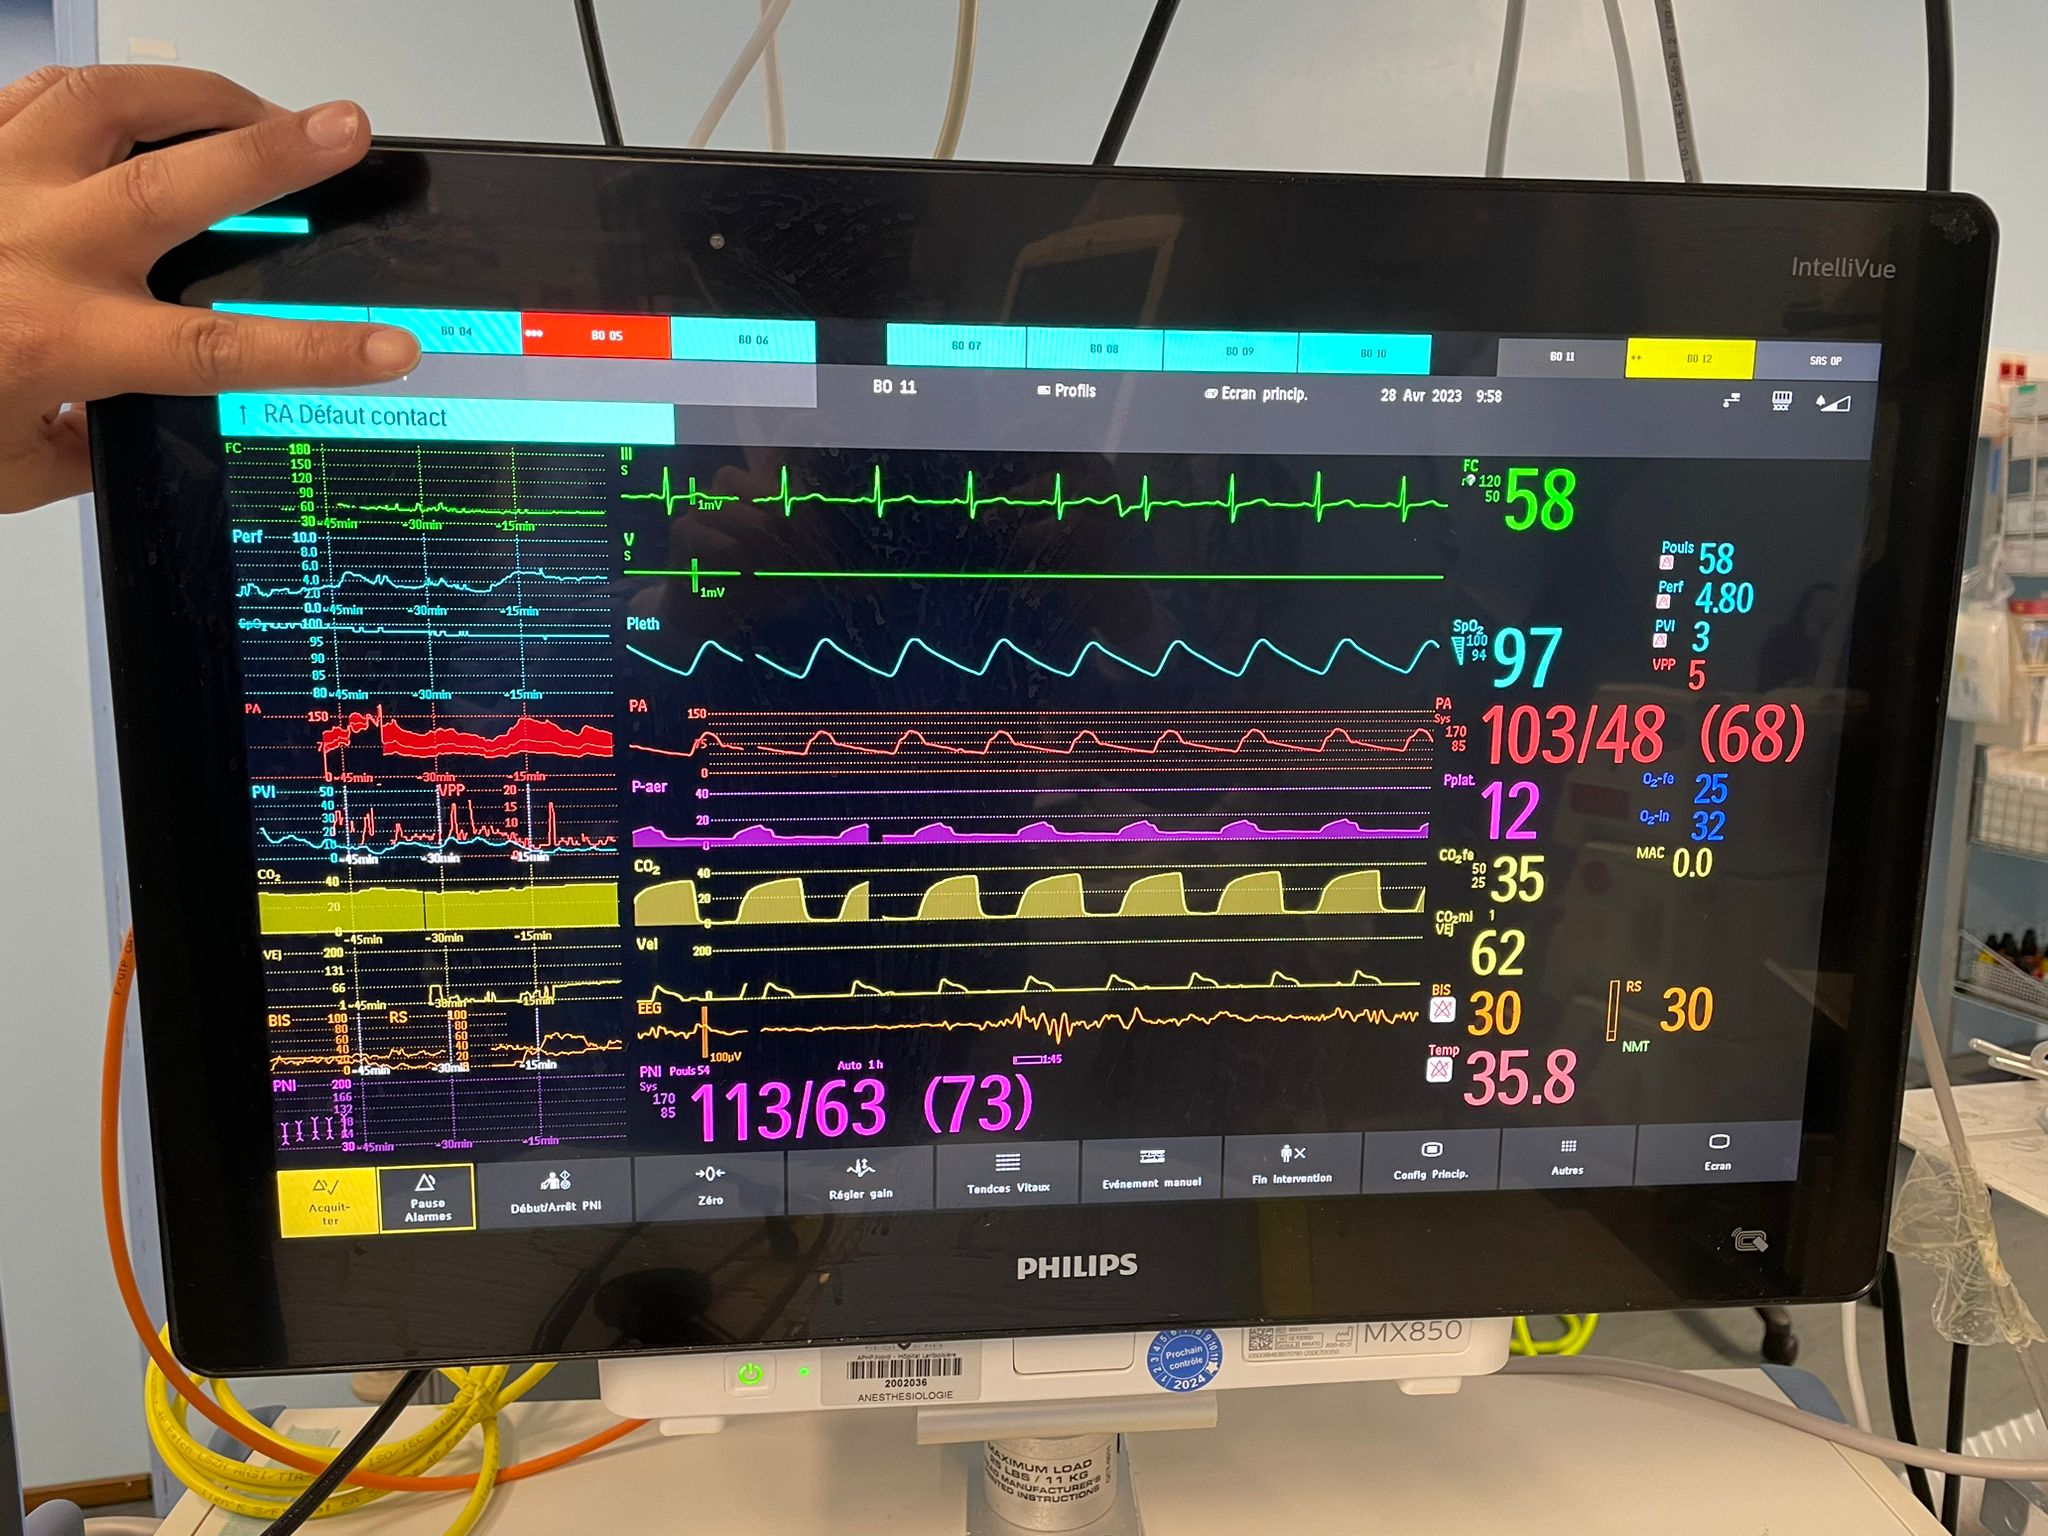
\includegraphics[
            width=1.16\paperwidth
        ]{GA_monitor_1}
    \end{picture}
}
\frame{
    \frametitle{Events-based processing}


    \setbeamercolor{events}{bg=darkred!50}
    \begin{tikzpicture}[overlay, remember picture]

        \node[anchor=east, yshift=7em, xshift=-3em] at (current page.east)
            (patterns) {\highlight[shadow=false]{
                % Signal's patterns
                % Underlying events
                Latent events
            }};

        \node[anchor=east, yshift=-2.5em] at (patterns.east) (ECG) {\highlight[shadow=false]{\color{black}\normalfont Heartbeat}};

        \node[rectangle, lightblue!70, draw=lightblue!70, very thick,
            minimum width=5ex,
            minimum height=2em, xshift=5.5ex, yshift=-7.8em]
                at (current page.north) (box_ecg) {};
        \draw[->, ultra thick, lightblue!70] ($(ECG.west)+(3ex, 0)$) -- (box_ecg.east);
        \node[anchor=south, xshift=.2ex, yshift=1em] at (box_ecg.west) (ecg_tip) {};
        \node[anchor=south, xshift=.2ex, yshift=-.8em] at (box_ecg.west) (ecg_base) {};
        \draw[-{Square[]}, ultra thick, green] (ecg_base) -- (ecg_tip) ;



        \node[anchor=east, yshift=-5em] at (patterns.east) (Pleth) {\highlight[shadow=false]{\color{black}\normalfont  Dichrote wave}};

        \node[rectangle, lightblue!70, draw=lightblue!70, very thick,
            minimum width=4ex,
            minimum height=2em, xshift=.2ex, yshift=-10.8em]
                at (current page.north) (box_pleth) {};
        \draw[->, ultra thick, lightblue!70] ($(Pleth.west)+(3ex, 0)$) -- (box_pleth.east);
        \node[anchor=south, xshift=.1ex, yshift=1.5em] at (box_pleth.west) (pleth_tip) {};
        \node[anchor=south, xshift=.1ex, yshift=-1em] at (box_pleth.west) (pleth_base) {};
        \draw[-{Circle[]}, ultra thick, blue] (pleth_base) -- (pleth_tip) ;

        \node[anchor=east, yshift=-7.5em] at (patterns.east) (Resp) {\highlight[shadow=false]{\color{black}\normalfont  Breath Cycle}};

        \node[rectangle, lightblue!70, draw=lightblue!70, very thick,
        minimum width=4ex,
        minimum height=2em, xshift=-2ex, yshift=-15.5em]
        at (current page.north) (resp_box) {};
        \draw[->, ultra thick, lightblue!70] ($(Resp.west)+(3ex, 0)$) -- (resp_box.east);
        \node[anchor=south, xshift=.2ex, yshift=1.5em] at (resp_box.west) (resp_tip) {};
        \node[anchor=south, xshift=.2ex, yshift=-1em] at (resp_box.west) (resp_base) {};
        \draw[-{Triangle[]}, ultra thick, yellow] (resp_base) -- (resp_tip) ;

        \node[anchor=east, yshift=-10em] at (patterns.east) (EEG) {\highlight[shadow=false]{\color{black}\normalfont  Brain waves}};

        \node[rectangle, lightblue!70, draw=lightblue!70, very thick,
        minimum width=6ex,
        minimum height=1.3em, xshift=-2ex, yshift=-17.8em]
        at (current page.north) (eeg_box) {};
        \draw[->, ultra thick, lightblue!70] ($(EEG.west)+(3ex, 0)$) -- (eeg_box.east);
        \node[anchor=south, xshift=.2ex, yshift=1.5em] at (eeg_box.west) (eeg_tip) {};
        \node[anchor=south, xshift=.2ex, yshift=-.6em] at (eeg_box.west) (eeg_box) {};
        \draw[-{Turned Square[]}, ultra thick, orange] (eeg_box) -- (eeg_tip) ;




        \node[anchor=west, xshift=0em, yshift=7em] at (current page.west)
            (events) {\highlight[shadow=false, col=events,c=white]{
                Observed events
            }};
        \node[anchor=west, yshift=-3.5em] at (events.west)
            {\highlight[shadow=false,col=events,c=black]{
                \normalfont Drug injection
            }};
        \node[anchor=west, yshift=-7em] at (events.west)
            {\highlight[shadow=false,col=events,c=black]{
                \normalfont Surgery acts
            }};
        \node[anchor=west, yshift=-10.5em] at (events.west)
            {\highlight[shadow=false,col=events,c=black]{
                \normalfont Adverse outcomes
            }};

    \end{tikzpicture}
}
}

%------------------------------------------------------------------------------

\frame{
    \frametitle{EBUL: Event-based Unsupervised Learning for Physiological Signals}


    \begin{block}{\bf EBUL Goal}
        Model the Distribution of Events for Physiological Signals.
    \end{block}

    \vskip1em

    {\bf Hyp.:} Events' time distribution $\mathbb P(\{t_k\}_k)$ is much simpler than $\mathbb P(X)$.\\[1em]

    {\bf Challenge:} Need to identify the events and model their distribution jointly.\\[1em]

    {\centering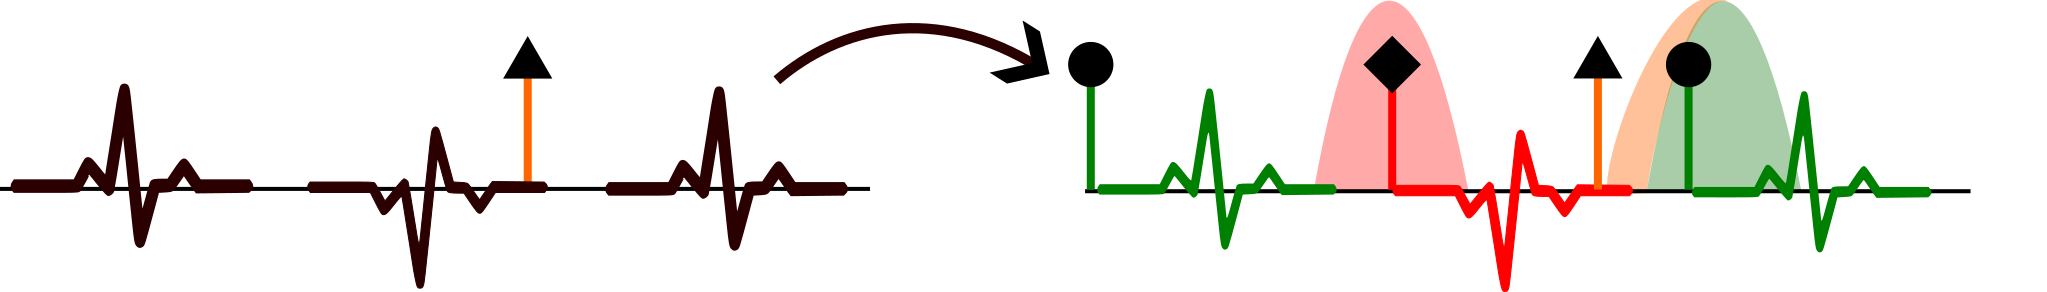
\includegraphics[width=.8\textwidth]{finding_events}\\[1em]}

    % {\bf Approach:} from interpretable models to deep learning.
    \pause
    \begin{columns}
        \hskip-1ex
        \column{.3\textwidth}
        \highlight{\parbox{\textwidth}{%
            \centering Events' distribution models\phantom{g}
        }}%
        \column{.3\textwidth}
        \highlight{\parbox{\textwidth}{%
            \centering Joint Modeling of Signals and Events
        }}%
        \column{.3\textwidth}
        \highlight{\parbox{\textwidth}{%
            \centering Task-specific Fine-tuning Algo.
        }}%
    \end{columns}
}

%------------------------------------------------------------------------------

\begin{frame}[t]{Beyond General Anesthesia Monitoring}

    \vskip-1em
    \begin{columns}[T]
        \column{.5\textwidth}
        \centering
        \begin{tikzpicture}
                \node[inner sep=0em, outer sep=0em] (img) {\includegraphics[width=.9\linewidth]{meg_signal}};
                \path let
                  \p1=($(img.north) - (0, 1em)$), \p2=(img.south)
                  in
                  node {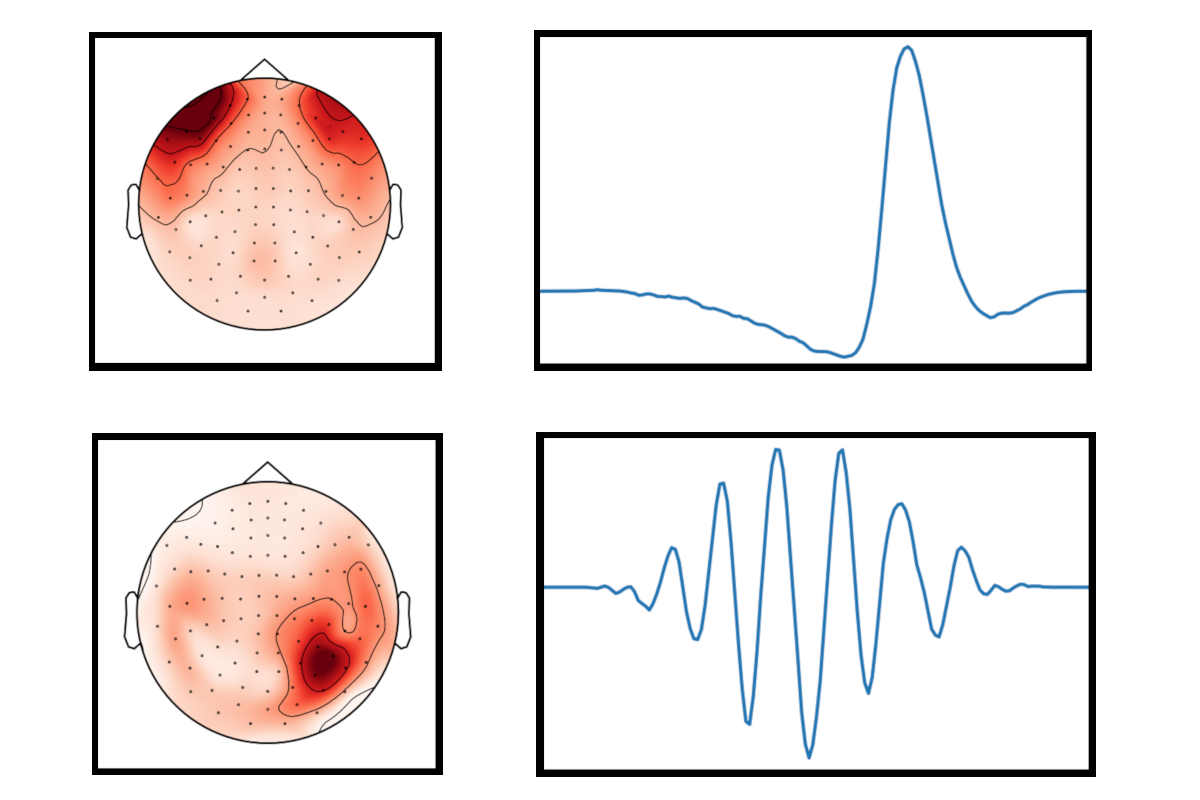
\includegraphics[height=\y1-\y2]{meg_dict}};
            \end{tikzpicture}\\
        {\large Neuroscience (MEG)}\\[1em]
        \begin{tikzpicture}
            \node[inner sep=0em, outer sep=0em] (img) {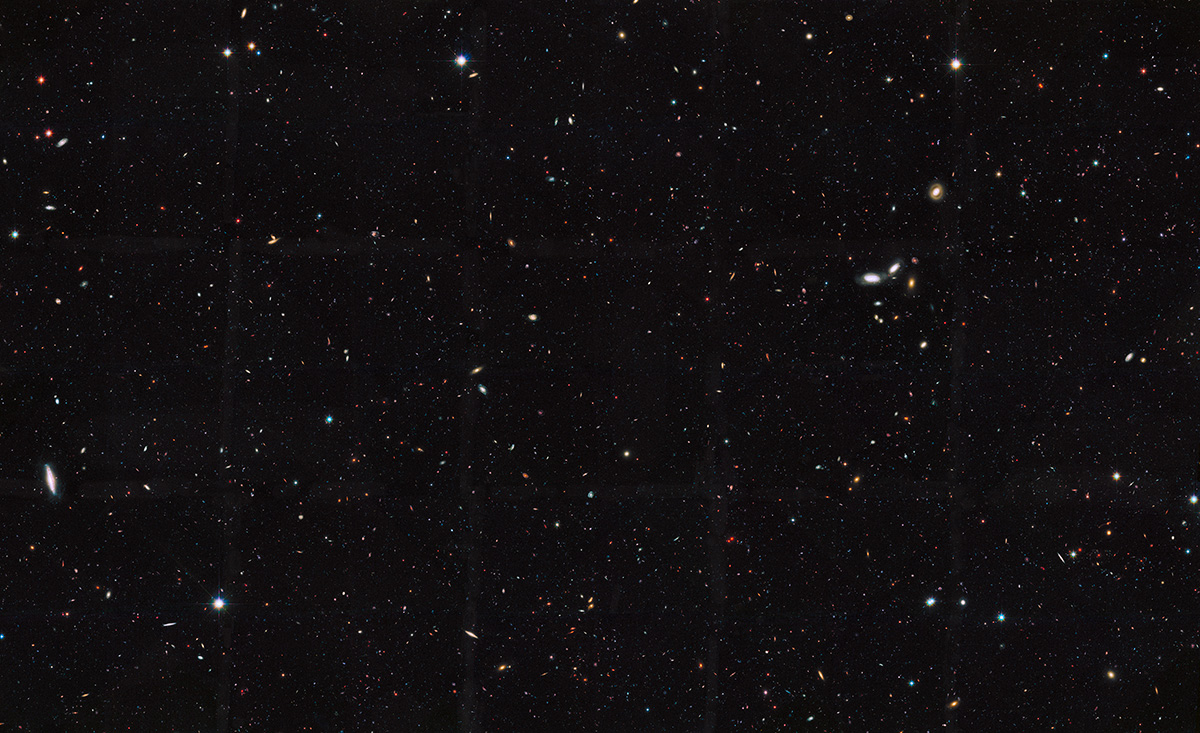
\includegraphics[width=.9\linewidth]{Hubble}};
            \path let
                \p1=($(img.north) - (0, 1em)$), \p2=(img.south)
                in
                node {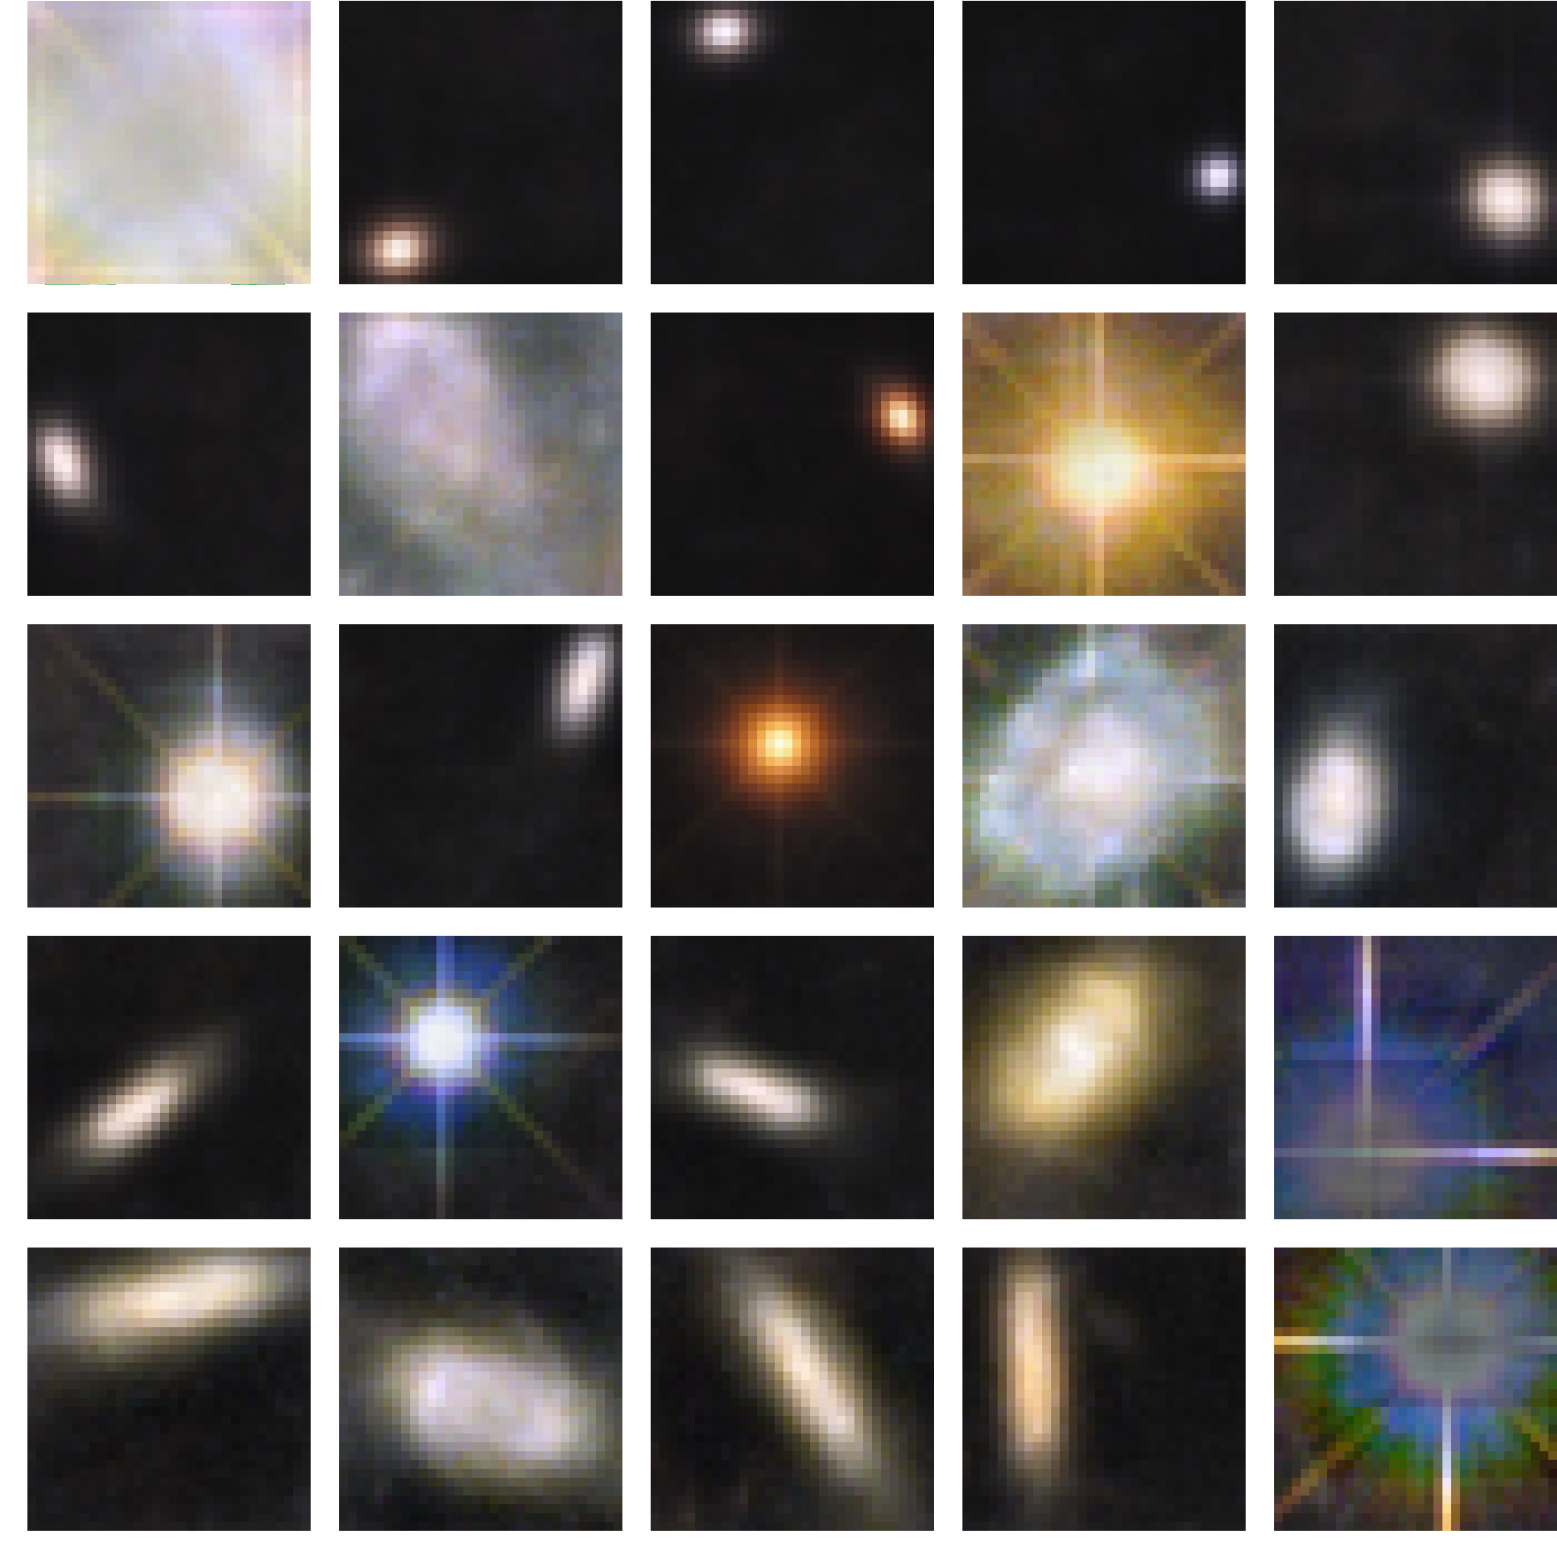
\includegraphics[height=\y1-\y2]{Hubble_dict}};
        \end{tikzpicture}\\
        {\large Astronomy}\\
    \column{.5\textwidth}
        \centering
        \begin{tikzpicture}
            \node[inner sep=0em, outer sep=0em] (img) {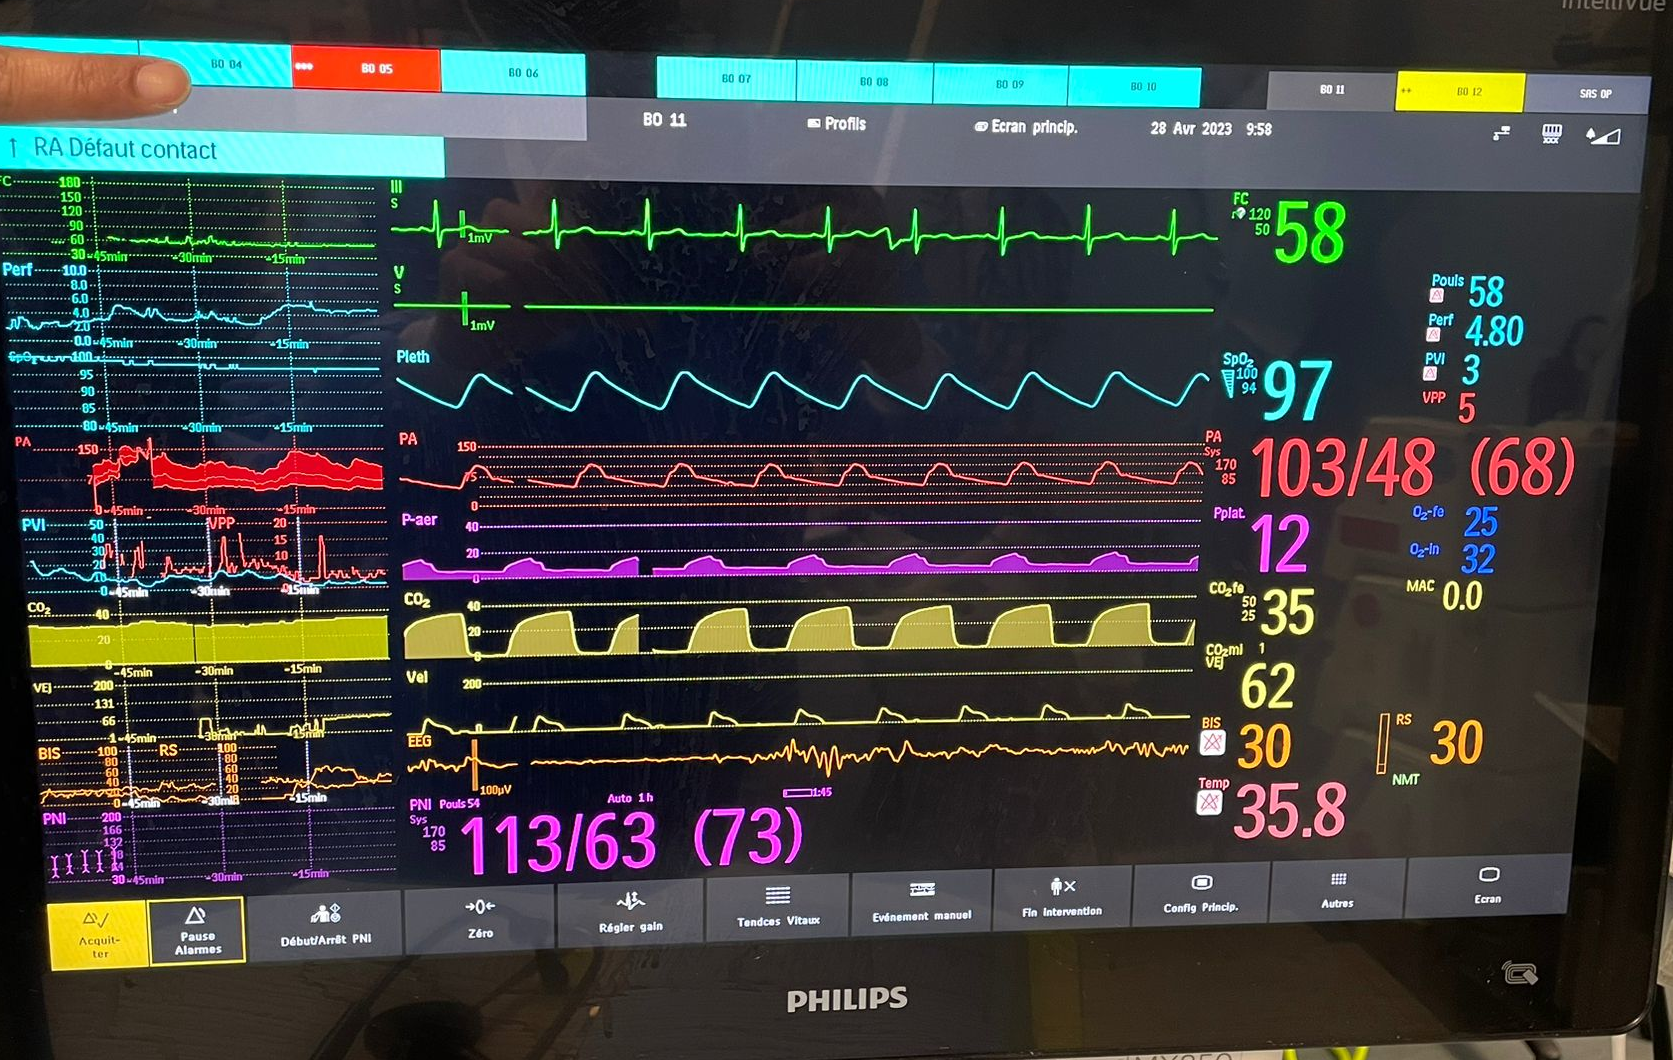
\includegraphics[width=.8\linewidth]{ga_signal}};
            \path let
                \p1=($(img.north) - (0, 1em)$), \p2=(img.south)
                in
                node {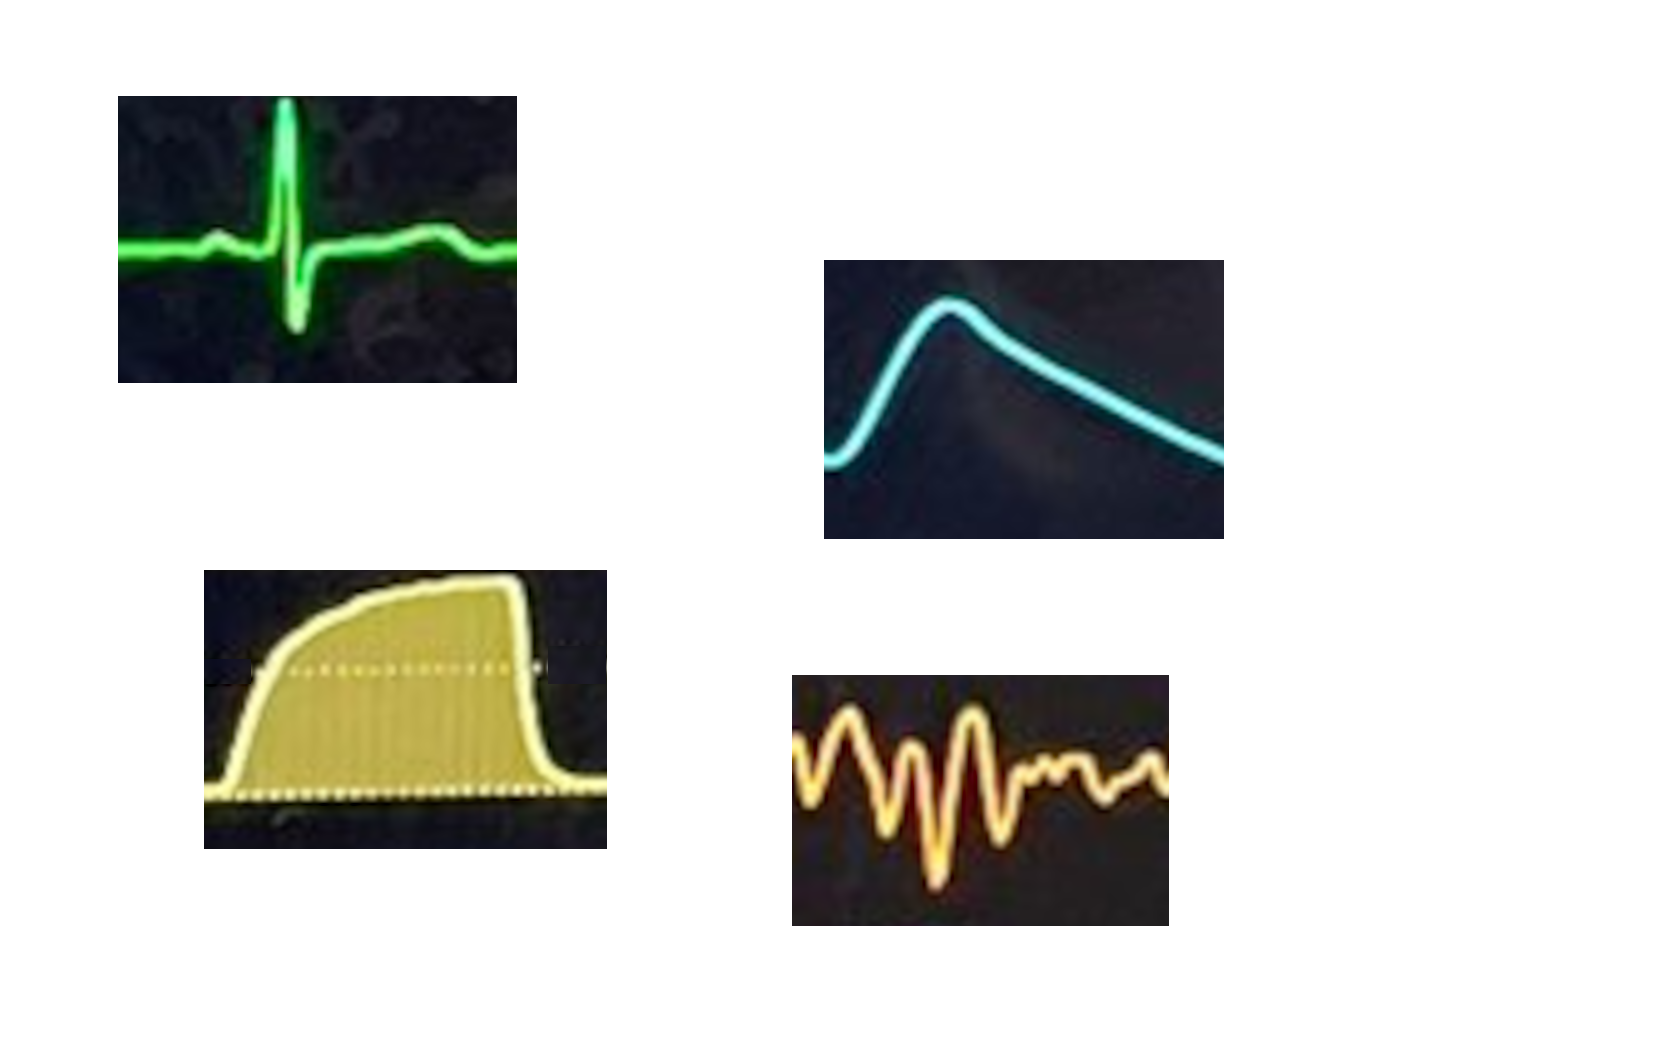
\includegraphics[height=\y1-\y2]{ga_dict}};
        \end{tikzpicture}\\
        {\large General Anesthesia}\\[1em]
        \begin{tikzpicture}
            \node[inner sep=0em, outer sep=0em] (img) {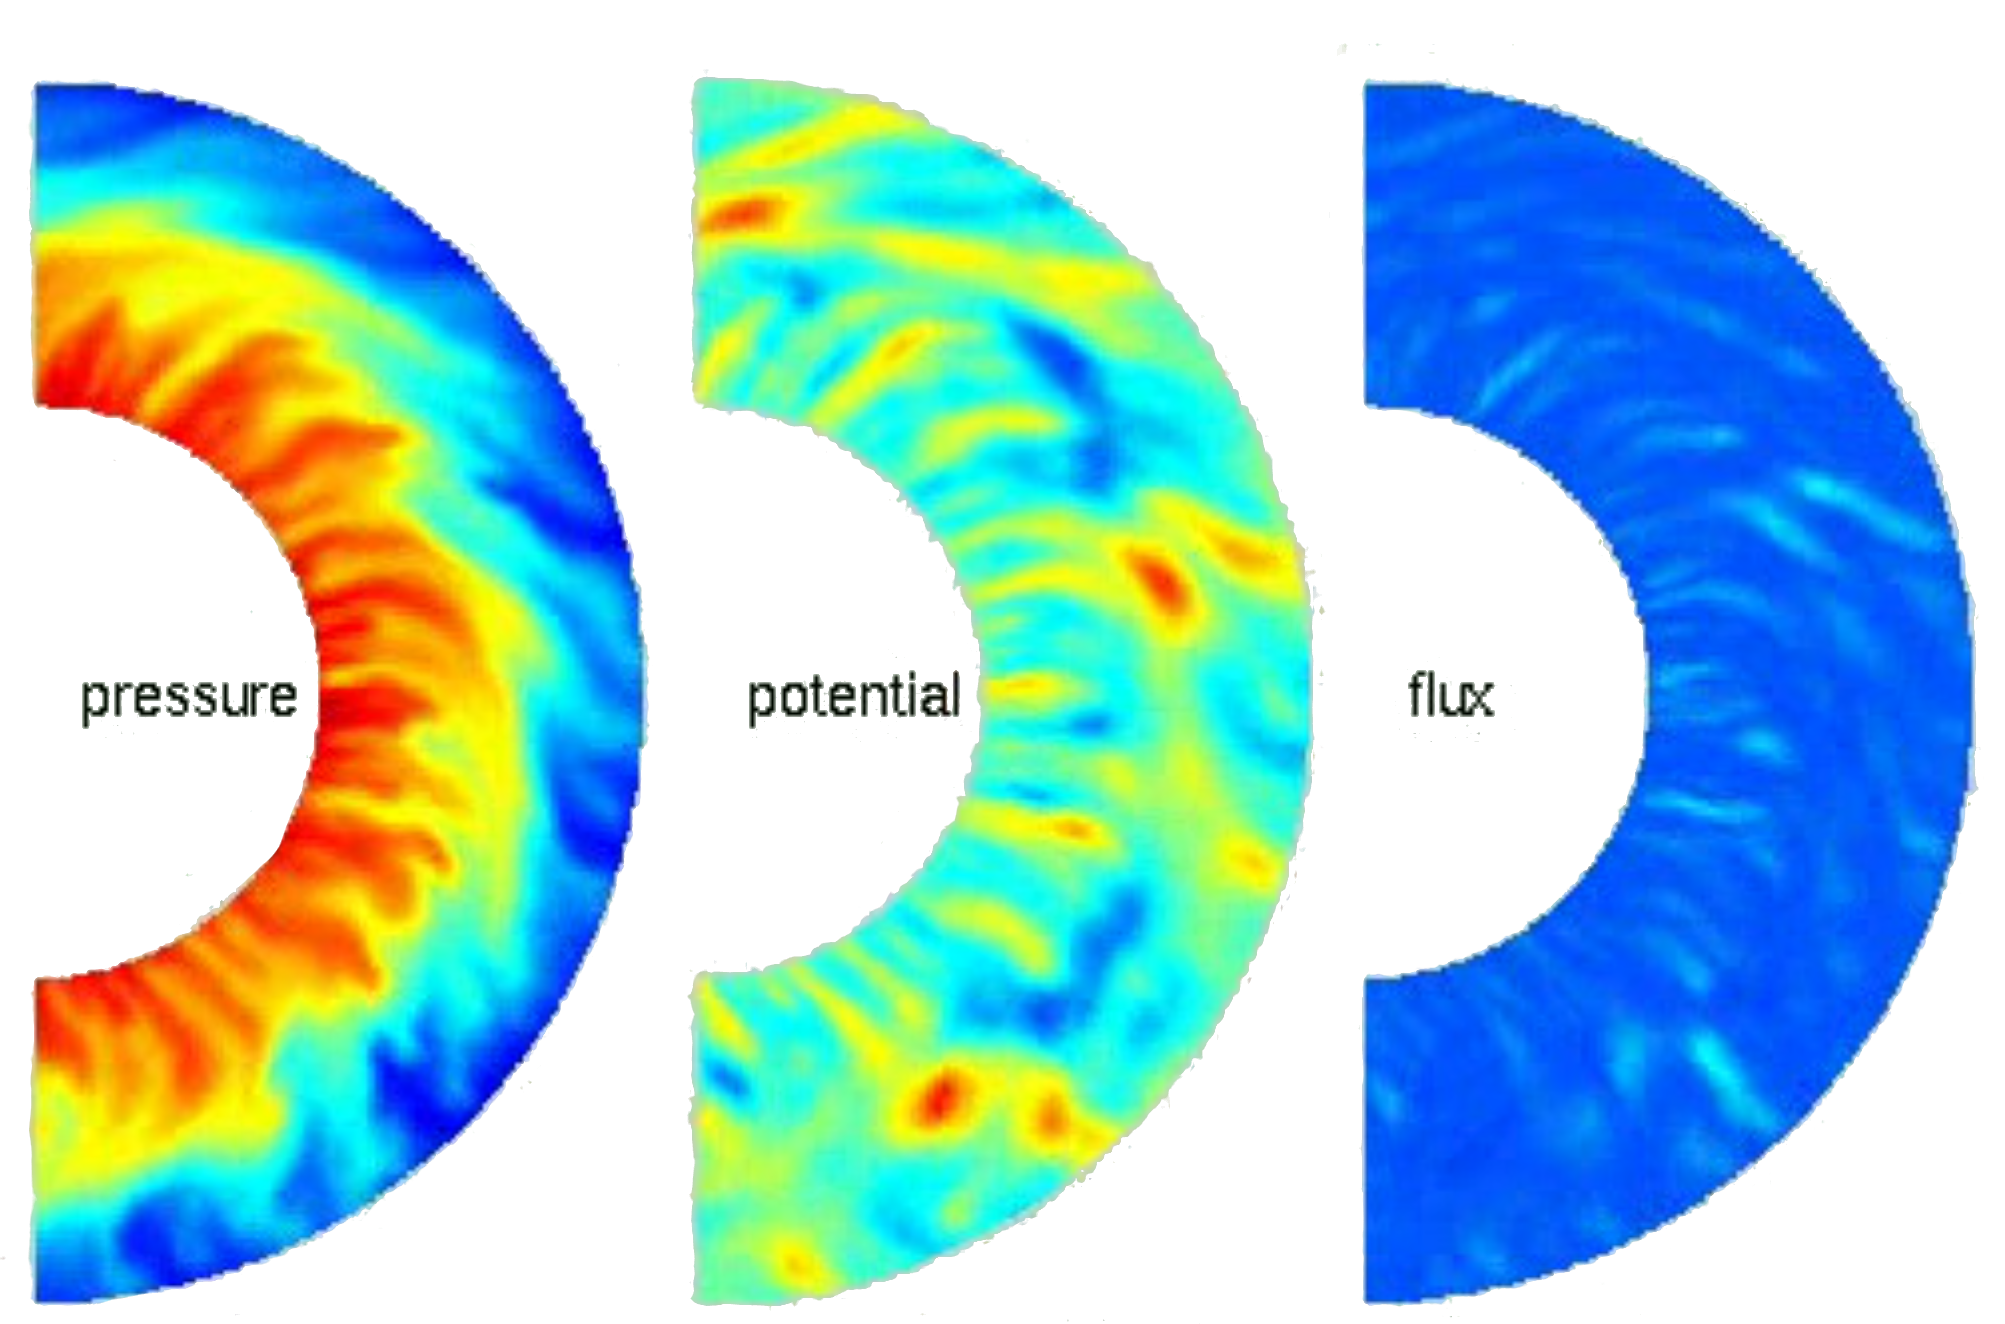
\includegraphics[width=.9\linewidth]{tokamak}};
            \path let
                \p1=($(img.north) - (0, 1em)$), \p2=(img.south)
                in
                node {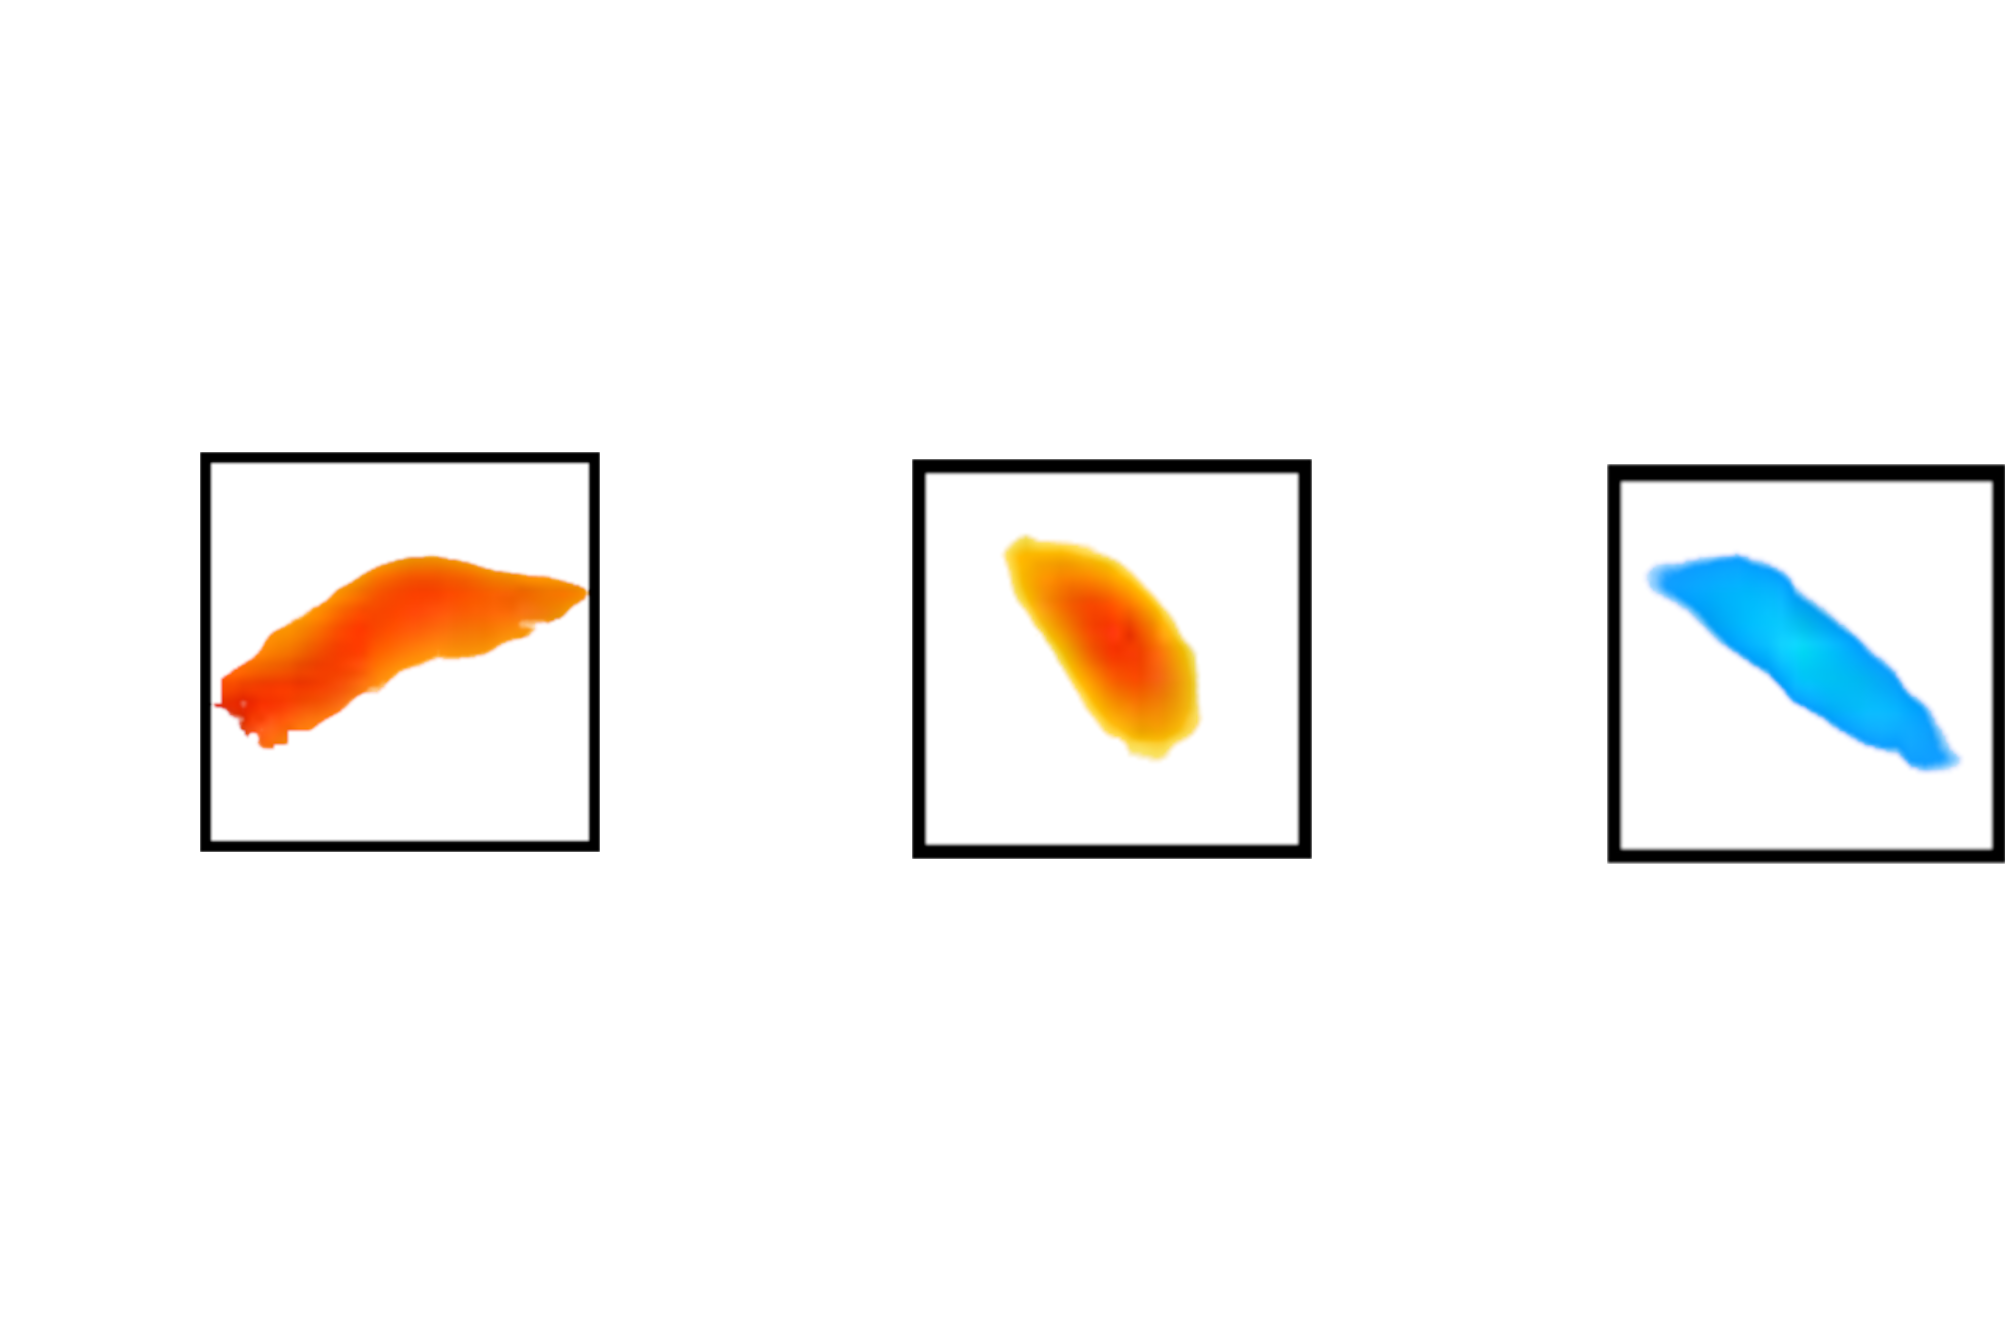
\includegraphics[height=\y1-\y2]{tokamak_dict}};
        \end{tikzpicture}\\
        {\large Physics Simulation}\\

    \end{columns}

    % \visible<2>
    {\vskip-14em
    \centering
    \highlight{\parbox{.35\textwidth}{
        \centering
        Latent Events\\
        are characterized by
        Recurring Patterns
    }}\\
    }
\end{frame}


\end{document}